\section{Interpretation}

The results of this search are interpreted in the context of several simplified models of dark matter as upper limits at a 95\% CL on the ratio of the signal cross section to the predicted cross section as a function of the mediator mass and and WIMP mass. The event samples for the simplified models are generated with \POWHEG V2 using the NNPDF30 PDFs. Various uncertainties in the experimental
acceptance are considered, for which typical magnitudes are summarised in Table~\ref{tab:signal_systs}.

\begin{table}[h!]
  \caption{%CMS {\it Simulation}. 
    Representative magnitudes of systematic uncertainties in the experimental
    acceptance for axial-vector mediated signal models.
  }
  \label{tab:signal_systs}
  \centering
%  \small
  \begin{tabular}{ lccc }
    \hline
    \hline
    Systematic source                   & Type          & Correlated & Typical magnitude (\%) \\
    \hline
    Luminosity                          & Normalisation & Yes        & 6.2                    \\
    Monte Carlo statistics              & Norm. + shape & No         & 1--50                  \\
    Jet energy scale                    & Norm. + shape & Yes        & 1--6                   \\
    b-tag efficiency scale factors      & Norm. + shape & Yes        & 0.4--0.8               \\
    Pile-up                             & Norm. + shape & Yes        & 0-2                    \\
    Trigger efficiency                  & Norm. + shape & Yes        & 0.0--0.3               \\
    Parton distribution functions       & Norm. + shape & Yes        & 1-3                    \\
    Factorisation/renormalisation scale & Norm. + shape & Yes        & 5-9                    \\
    \hline
    \hline
  \end{tabular}
\end{table}
  
%\begin{figure*}[thp!]
%  \begin{center}
%    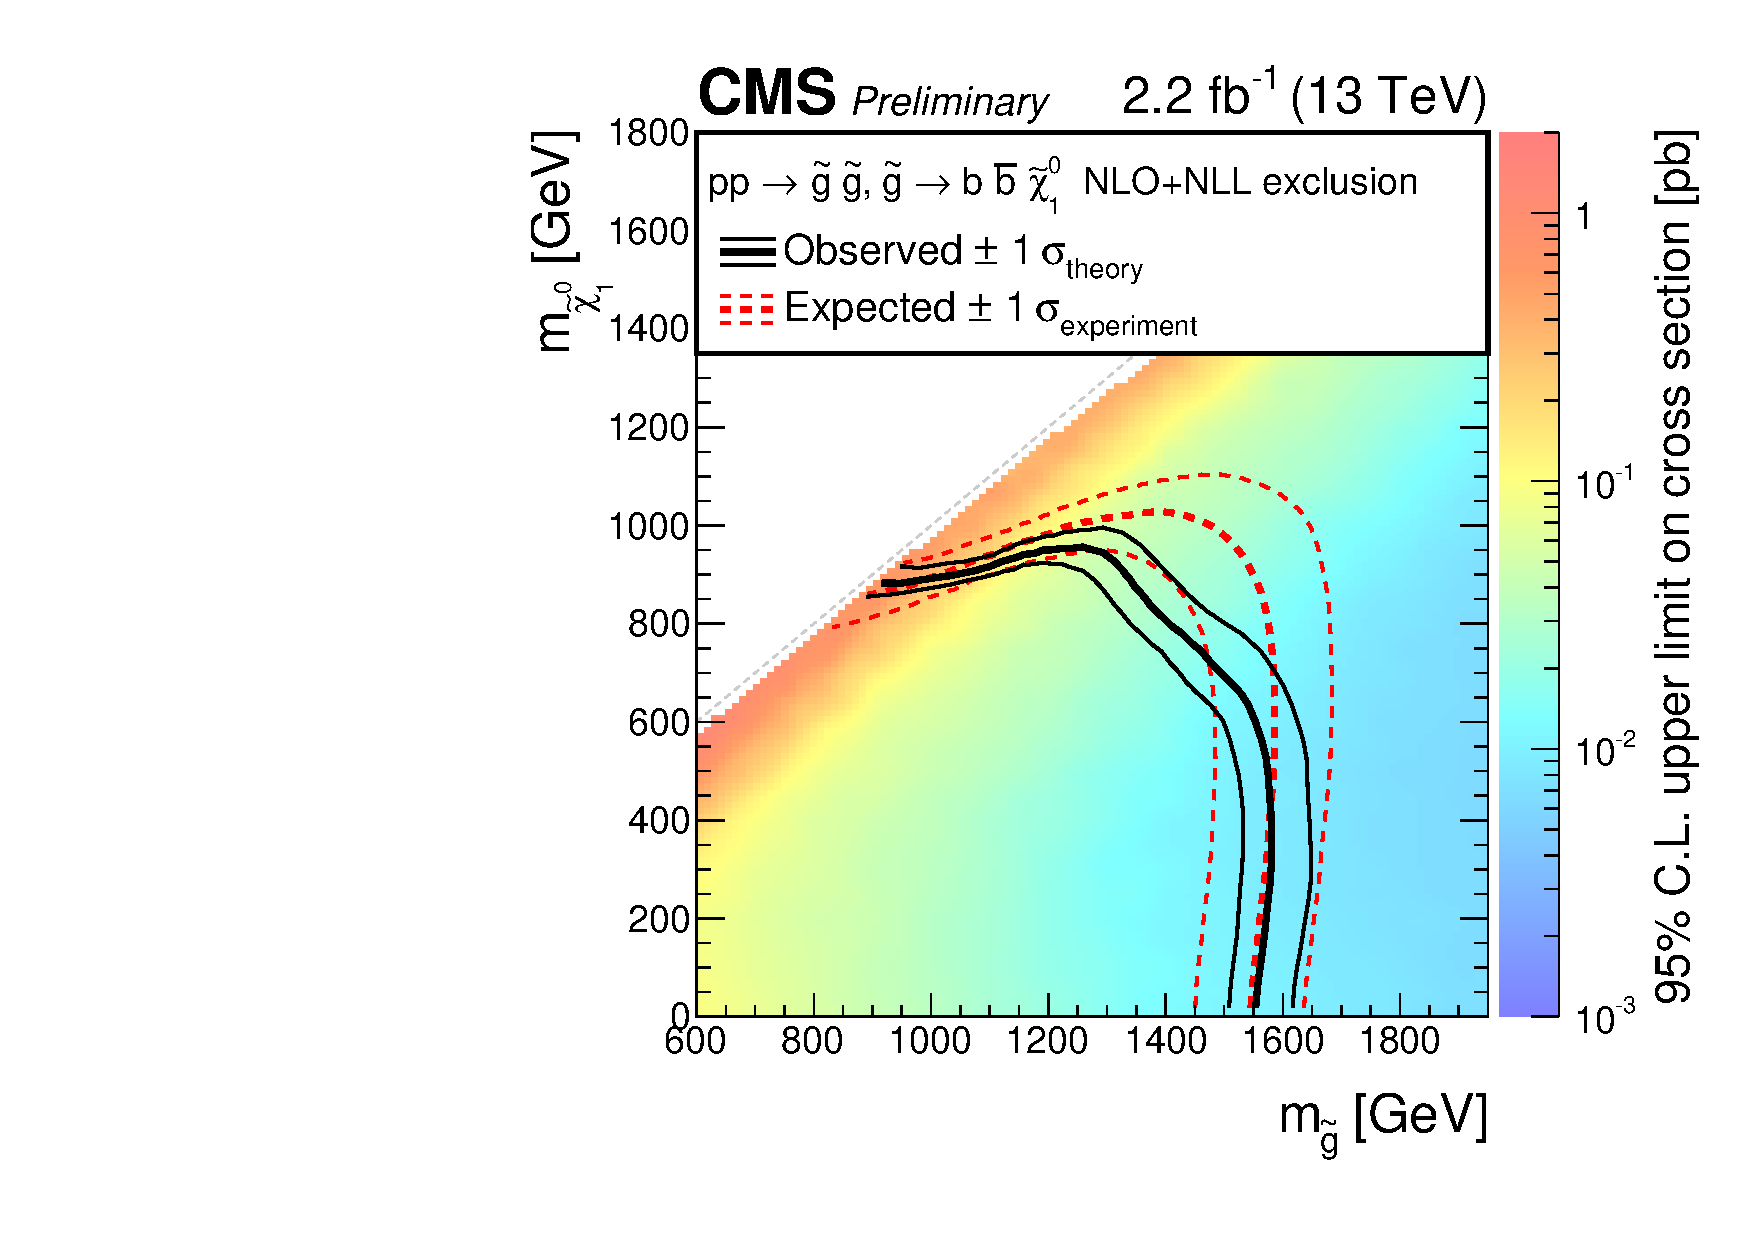
\includegraphics[width=0.49\textwidth]{t1bbbbRA1XSEC.pdf} \,
%    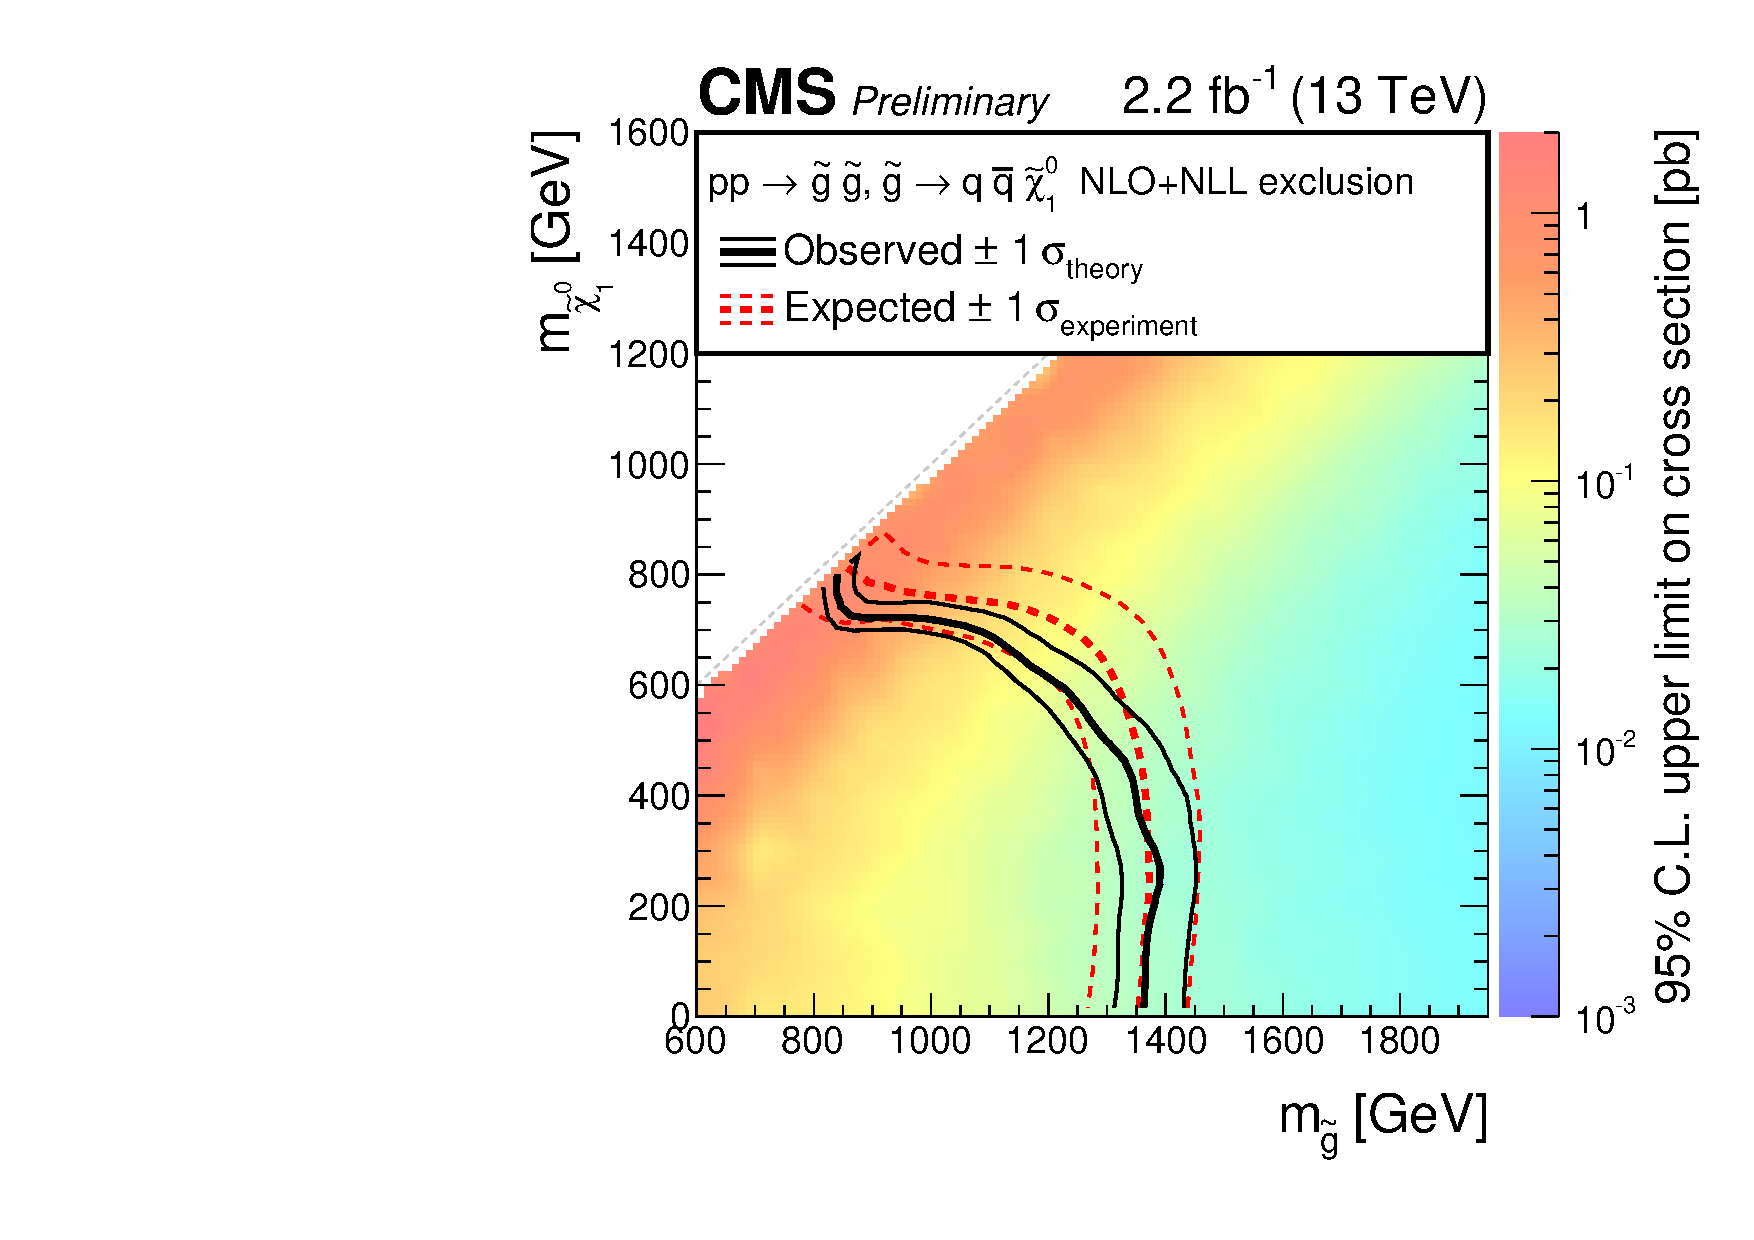
\includegraphics[width=0.49\textwidth]{t1qqqqRA1XSEC.pdf} \\
%    \caption{Observed upper limit in cross section at 95\% CL
%      (indicated by the colour scale) for simplified models that
%      assume the pair production of gluinos, as a function of the
%      gluino and $\chiz_{1}$ masses for gluino three-body decays to
%      $b\bar{b}\chiz_{1}$ (left) and $q\bar{q}\chiz_{1}$ (right). The
%      black solid thick (thin) line indicates the observed mass
%      exclusion region assuming the nominal (${\pm}1 \sigma$ theory
%      uncertainty) production cross section. The red dashed thick
%      (thin) line indicates the median (${\pm}1 \sigma$ experimental
%      uncertainty) expected exclusion.
%      \label{fig:limits-sms} }
%  \end{center}
%\end{figure*}

Figure~X \fixme{\it will show} 
%\ref{fig:limits-sms} shows 
the expected and observed upper limit on the
production cross section at 95\% confidence level (CL) as a function
of the mediator and WIMP masses for a range of simplified models assuming
pair production of WIMPs in association with jets originating from light flavour and heavy flavour quarks. The couplings of the mediator to SM particles is assumed to be 0.25 for the axial vector and vector models and 1.0 for the scalar and pseudoscalar models. The couplings of the mediator to WIMPs is assumed to be 1.0 for all models. 
Upper limits at 95\% CL are also presented on the cross section times branching fraction of the production via gluon fusion of the 125 GeV Higgs boson decaying to a pair of invisible particles. 

Table shows the expected 95\%CL limits for some signal points for a range of simplified models. 
\begin{table}[h!]
  \caption{%CMS {\it Simulation}. 
    95\% CL limits for a signal point in each of the four light flavour simplified models. }
  \label{tab:limits}
  \centering
%  \footnotesize
  \begin{tabular}{ lcc }
    \hline
    \hline
    Simplified model              & M$_{med}$,M$_{DM}$          & r-value (expected) \\ \hline
Vector & 1500,150 & 2.18 \\
Axial-vector & 1500,250 & 2.43 \\
Pseudo-scalar & 300,100 & 2.539 \\
Scalar & 300,1 & 3.64 \\
    \hline
    \hline
  \end{tabular}
\end{table}



%%__________________________________________________________________||
